% =====================================================================
%  chunks/ch02c.tex —— 原书 p.32–40 顶部（PDF 39–47 上半）
%  第 2 章 §4 收尾：纤维化正合列的重要特例、单值与覆叠、Example 1–8、Hopf 纤维化
%  本块止于第 3 章章标题之前（章标题在原书 p.40 中部），故块内不含 \chapter。
% =====================================================================
% [原文 p.32]
\begin{equation}
  \begin{aligned}
    \cdots\to\pi_n(F_0,x_0)&\to\pi_n(X,x_0)\xrightarrow{p_*}\pi_n(Y,y_0)
    \xrightarrow{\partial}\pi_{n-1}(F_0,x_0)\\
    &\to\pi_{n-1}(X,x_0)\to\cdots.
  \end{aligned}
  \tag{4.7}
\end{equation}

\para{重要的特例}
1. 设 $p:X\to Y$ 是覆叠空间投影（见上文），其（离散）纤维为 $F_0$。由于 $i\ge1$ 时 $\pi_i(F_0,x_0)=0$（$0$ 表示平凡群），正合列 (4.7) 在此情形下成为
\[
  \begin{aligned}
    \text{对 } n>1,&\quad 0\to\pi_n(X,x_0)\xrightarrow{p_*}\pi_n(Y,y_0)\to 0;\\
    \text{对 } n=1,&\quad 0\to\pi_1(X,x_0)\to\pi_1(Y,y_0)
    \xrightarrow{\partial}\pi_0(F_0,x_0)\to 0.
  \end{aligned}
\]
于是由正合性得到
\begin{equation}
  \pi_n(X,x_0)\cong\pi_n(Y,y_0),\qquad n>1, \tag{4.8}
\end{equation}
而在 $n=1$ 的情形，$\pi_1(X,x_0)$ 同构于 $\pi_1(Y,y_0)$ 的一个子群，并且其左陪集之集与纤维的分支数「同构」（即一一对应）；换言之，每个陪集对应于覆叠的一个叶。

2. 考虑任意空间 $Y$ 上的 Serre 纤维化；于是这里（如前）全空间 $X=E_{y_0}$ 是所有始于点 $y_0=\gamma(a)$ 的道路 $\gamma(t)$（$a\le t\le b$）之空间。显然 $X$ 可缩。所选点 $y_0$ 上方的纤维 $F_0=p^{-1}(y_0)$ 是环路空间 $\Omega(y_0)$，它由所有始于并终于 $y_0$ 的闭道路组成。对这个纤维化，正合列 (4.7) 给出
\[
  0\to\pi_n(Y,y_0)\xrightarrow{\partial}\pi_{n-1}(\Omega(y_0),x_0)\to 0,
  \qquad n\ge1,
\]
由此得到同构
\begin{equation}
  \pi_n(Y,y_0)\cong\pi_{n-1}(\Omega(y_0),x_0), \tag{4.9}
\end{equation}
其中 $x_0$ 表示像为点 $y_0$（对一切 $t$）的平凡环路。这个同构实际上被 Hurewicz 用来递归地定义同伦群。\hfill$\square$
% [Tutor Note: 特例 1 里 (4.8) 的 $n>1$ 版依赖「覆叠的纤维离散」这一条；纤维一旦有非平凡同伦型，$p_*$ 就一般不再是同构。特例 2 把 (4.7) 反过来用：$E_{y_0}$ 可缩使两端群为零，剩下的 $\partial$ 只能是同构，这就是「环路空间降一次」的来历。]

% [Tutor Note: 特例 1 中「陪集之集与纤维分支数同构」一句，原书给「同构」加了引号，因为这里谈的不是群同构，而是集合间的一一对应：$\pi_1(Y,y_0)/p_*\pi_1(X,x_0)$ 的每个陪集恰对应覆叠的一个叶（分支）。]

重新回到任意纤维化 $p:X\to Y$，我们回想基本假设：纤维化带有「同伦联络」。特别地，这使我们能沿底空间中的道路搬运纤维；也就是说，底空间中每条道路 $\gamma(t)$（$a\le t\le b$）都对应一个纤维之间的映射
\[
  \tilde\gamma:F_0\to F_1,\qquad F_0=p^{-1}(y_0),\quad F_1=p^{-1}(y_1),
\]
\[
  y_0=\gamma(a),\qquad y_1=\gamma(b),
\]
它连续依赖于道路 $\gamma$。以 $y_0$ 为起点和终点的闭道路 $\gamma$，就这样给出一个同伦等价
\[
  \tilde\gamma:F_0\to F_0,
\]
而后者又在第 $n$ 个同伦群之间诱导出「单值性」（monodromy）同构：
% [原文 p.33]
\[
  \tilde\gamma_*:\pi_n(F_0,x_0)\to\pi_n(F_0,\tilde\gamma(x_0)).
\]
我们在第 1 章讨论 Riemann 曲面时遇到过这一现象的特例：那里 $n=0$，底空间是 $\R^2$ 的一个区域，而记作 $\sigma_\gamma$ 的单值性是离散纤维的一个置换。

值得在所有覆叠空间类中挑出\emph{正规}覆叠，即像 $p_*\pi_1(X)\subset\pi_1(Y)$ 是 $\pi_1(Y)$ 的正规子群的那些覆叠空间。对这样的覆叠空间，商群 $\pi_1(Y)/p_*\pi_1(X)=\Gamma$ 自然地作为空间 $X$ 的一个离散变换群（自同胚群）作用：作用通过沿底空间 $Y$ 中的闭道路 $\gamma$ 搬运纤维来定义，即通过单值性来定义；而那些同伦类落在像 $p_*\pi_1(X)$ 中的道路给出平凡的单值性。
% [Tutor Note: 这一段的「正规」判据是覆叠分类的中心结论：正规覆叠对应 $\pi_1(Y)$ 的正规子群，一般覆叠只对应子群。空间 $X$ 上的这个变换群就是覆叠的「deck 变换」群；原书把作用写在左边、把商写成 $\pi_1(Y)/p_*\pi_1(X)$，与「左作用配左陪集」的约定一致。]

给定空间 $Y$ 的最大覆叠空间 $X$ 称为 $Y$ 的\emph{万有覆叠空间}。可以证明，对很大一类空间 $Y$，它存在且唯一。空间 $X$ 是单连通的：$\pi_1(X)$ 平凡，因此按上面的讨论它是正规覆叠，而 $\Gamma=\pi_1(Y)$ 自然地离散地作用于它，轨道恰为纤维 $p^{-1}(y)$。由于 $X$ 单连通，它的同伦群不依赖于基点 $x_0$。群 $\Gamma$（它离散且自由地作用于 $X$，即只有单位元固定任何点）诱导同态
\[
  \gamma:\pi_n(X)\to\pi_n(X),\qquad n>1,\ \gamma\in\Gamma.
\]
注意到 $\Gamma=\pi_1(Y,y_0)$，我们于是得到 $\pi_1$ 在一切 $\pi_n$ 上的作用，并且具有自然的几何解释。

\begin{example}{1}
设 $U\subset\R^3$ 是从 $\R^3$ 中去掉一条直线以及该直线外一个点后所得的区域。区域 $U$ 则以圆周与 2 维球面的楔和为形变收缩核：
\[
  U\sim S^2\vee S^1=Y.
\]
容易推出 $\pi_1(U)=\pi_1(S^2\vee S^1)\cong\Z\cong\pi_1(S^1)$，其中 $\Z$ 是无限循环群，其生成元记作 $t$。考虑 $U$ 的万有覆叠，或者更确切地说，考虑楔和 $S^2\vee S^1=Y$ 的同伦等价的万有覆叠 $X$：
\[
  X\to Y=S^2\vee S^1.
\]
空间 $X$ 可以表示成直线 $\R$（坐标记为 $\lambda$）在每个整数点 $j$ 处粘上一个 2 维球面 $S_j^2$（见图 2.16）。$\pi_1(Y)$ 在 $X$ 上的作用此时由
\begin{equation}
  t(\lambda)=\lambda+1,\qquad t(S_j^2)=S_{j+1}^2 \tag{4.10}
\end{equation}
给出。
\begin{figure}[htbp]
  \centering
  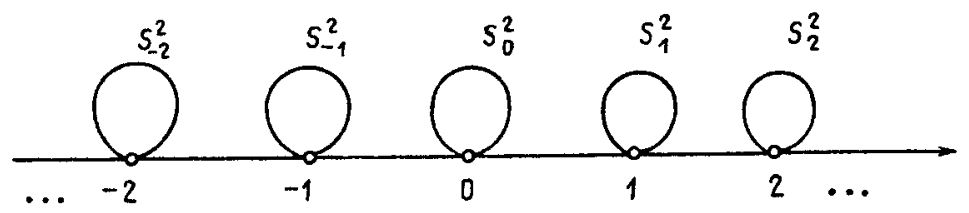
\includegraphics[width=0.72\textwidth]{figures/fig2_16.png}
  \figtitle{2.16}{}
\end{figure}
% [原文 p.34]
空间 $X$ 的 2 维同伦群 $\pi_2(X)$ 是可数无限多个 $\Z$ 的直和，其基记作 $\{d_j\}$，每个 $d_j$ 由显然的映射 $S^2\to S_j^2$ 几何地定义。$\pi_1(Y)$ 在 $\pi_2(X)$ 上的作用于是显然由
\begin{equation}
  t(d_j)=d_{j+1} \tag{4.11}
\end{equation}
给出。鉴于同构 (4.8)，这也描述了 $\pi_2(S^2\vee S^1)\cong\pi_2(U)$ 的结构，包括 $\pi_1(S^2\vee S^1)\cong\Z$ 在它上面的作用。用模的语言说，$\pi_2(U)$ 于是是以 $d=d_0$ 为唯一生成元的自由 $\Z[\pi]$-模（$\pi=\pi_1(U)$），因为 $\pi_2(U)$ 的每个元素 $a$ 都有唯一的形式
\[
  a=\sum_{j=-N}^{+M}\lambda_j t^j(d),
\]
其中 $\lambda_j$ 是整数，$\sum\lambda_j t^j\in\Z[\pi]$，且 $\pi=\pi_1(Y,y_0)$。
\end{example}
% [Tutor Note: 这个例子是全书第一次把 $\Z[\pi]$-模结构具体算出来：$t$ 可逆，故 $\Z[\pi]=\Z[t,t^{-1}]$（Laurent 多项式环），而 $\pi_2(U)$ 就是它作为自身上的自由模。「唯一形式」里的 $\sum_{j=-N}^{+M}$ 允许有限个负幂，这正对应 $t$ 在 $\pi$ 中可逆。]

\begin{example}{2}
实射影平面 $\RP^2$ 的点是非零实向量 $(\lambda^0,\lambda^1,\lambda^2)$ 的等价类，其中两个三元组等价当且仅当一个是另一个的非零纯量倍：
\[
  (\lambda\lambda^0,\lambda\lambda^1,\lambda\lambda^2)\sim(\lambda^0,\lambda^1,\lambda^2),
  \qquad \lambda\ne0;
\]
换言之，$\RP^2$ 的点是 $\R^3$ 中过原点的直线（原点已去掉）。加上单位长度的要求，每个等价类恰有两个代表：
\[
  \sum_{j=0}^2(\lambda^j)^2=1.
\]
由此清楚，$\RP^2$ 可以看作 2 维球面 $S^2$ 上 2 阶离散群 $\Z/2$ 作用的轨道空间：
\[
  (\lambda^0,\lambda^1,\lambda^2)\sim(-\lambda^0,-\lambda^1,-\lambda^2).
\]
由于群 $\pi_1(S^2)$ 平凡，这个覆叠对 $\RP^2$ 是万有的。由 (4.8) 我们有
\begin{equation}
  \pi_2(S^2)\cong\pi_2(\RP^2)\cong\Z. \tag{4.12}
\end{equation}
% [原文 p.35]
把 $\pi_2(\RP^2)$ 的一个生成元记作 $d$。鉴于上面把 $\RP^2$ 描述为其万有覆叠在 $\Z/2$ 作用下的轨道空间，我们还有 $\pi_1(\RP^2)\cong\Z/2$；把 $\pi_1(\RP^2)$ 的生成元记作 $t$，$t^2=1$，它可以看作在球面 $S^2$ 上适当地作用。$\pi_2(\RP^2)$ 作为 $\Z[\pi_1]$-模的结构于是由
\begin{equation}
  t(d)=-d,\qquad t^2=1 \tag{4.13}
\end{equation}
给出。
容易证明 $i<n$ 时 $\pi_i(S^n)=0$，且 $\pi_n(S^n)=\Z$。与刚处理的 $n=2$ 情形大致相同，可以推出 $n$ 维实射影空间 $\RP^n$ 满足
\begin{equation}
  \pi_i(\RP^n)\cong\pi_i(S^n),\quad i>1;\qquad
  \pi_1(\RP^n)\cong\Z/2. \tag{4.14}
\end{equation}
此外，群 $\pi_1(\RP^n)$ 的生成元 $t$ 按如下公式作用在 $\pi_n(\RP^n)$ 的基元素 $d$ 上（把它看作 $\Z[\pi_1]$-模）：
\begin{equation}
  t(d)=(-1)^{n+1}d, \tag{4.15}
\end{equation}
其中因子 $(-1)^{n+1}$ 来自 $\R^{n+1}$ 的反射 $x\to-x$ 限制到球面 $S^n\subset\R^{n+1}$ 上时对定向的影响。
最后我们指出，对空间 $\RP^\infty$（定义为空间序列 $\RP^n$，$n=1,2,\dots$ 的直接极限，其中每个空间自然地嵌入其后继），基本群仍是 $\Z/2$，而各群 $\pi_i(\RP^\infty)$（$i>1$）全都平凡。
\end{example}
% [Tutor Note: (4.13) 与 (4.15) 的符号差别正是「定向」在起作用：$\RP^n$ 可定向当且仅当 $n$ 为奇数，此时对径映射在 $\pi_n$ 上保向；$n$ 为偶数时反号。读者易把 $(-1)^{n+1}$ 误写成 $(-1)^n$，可用 $n=2$ 校验：$\RP^2$ 不可定向，$t(d)=-d$，而 $(-1)^{2+1}=-1$，相符。]

\begin{example}{3}
每个连通的平面区域（或者更一般地，每个开 2 维流形）都以某个一维复形为形变收缩核。每个一维复形都同伦等价于有限个或可数无限多个圆周的楔和。（后一情形可方便地实现为图 2.17(c) 中所示的复形。）
\begin{figure}[htbp]
  \centering
  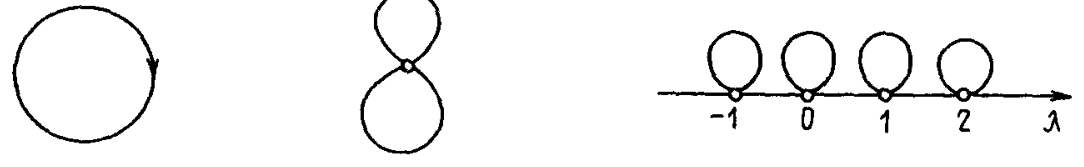
\includegraphics[width=0.80\textwidth]{figures/fig2_17.png}
  \figtitle{2.17}{(a) 圆周；(b) 楔和；(c) 在 $\lambda$ 轴的整数点 $\lambda=n$ 处粘上的圆周}
\end{figure}
% [原文 p.36]
例如，楔和 $S^1\vee S^1$ 以图 2.18 所示的树为其万有覆叠。要看出这一点，注意覆叠图中的每个顶点都位于楔和的唯一顶点上方，因此它的某个邻域必定同胚于楔和顶点的某个邻域，即同胚于一个「十字」。在这棵树上，两个生成元的自由群自然地自由作用，轨道空间就是楔和 $S^1\vee S^1$。由这类论证可知，对每个一维复形（或图）$K$，$\pi_1(K)$ 都是自由群。
\begin{figure}[htbp]
  \centering
  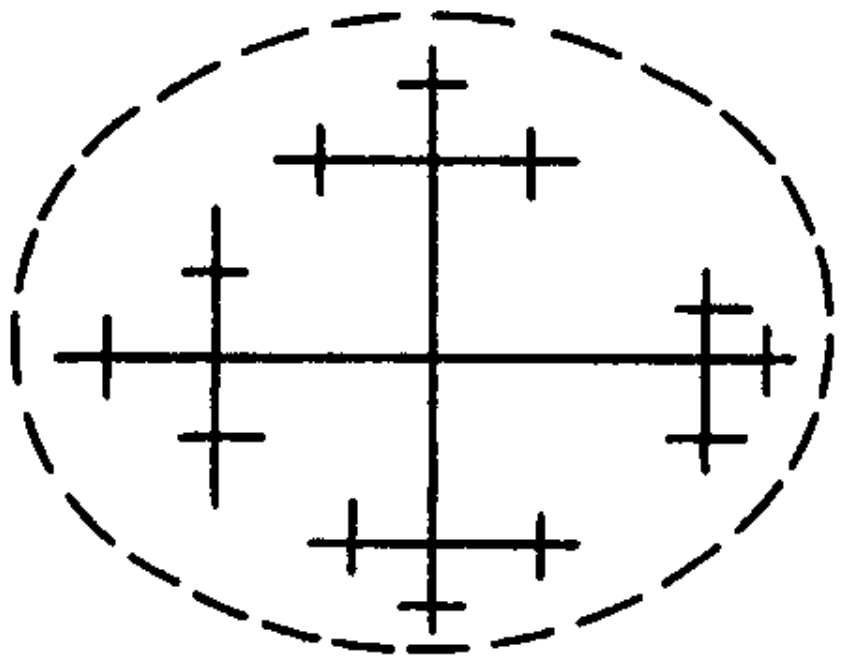
\includegraphics[width=0.42\textwidth]{figures/fig2_18.png}
  \figtitle{2.18}{$S^1\vee S^1$ 的万有覆叠树}
\end{figure}
\end{example}

\begin{example}{4}
$n$ 维环面 $T^n$ 由 $\R^n$ 通过如下等同得到：
\[
  (\lambda^1,\dots,\lambda^n)\sim(\bar\lambda^1,\dots,\bar\lambda^n),
\]
只要 $(\lambda^1-\bar\lambda^1,\dots,\lambda^n-\bar\lambda^n)$ 的各个分量都是整数。我们立刻推出整数格 $\Z^n$ 在 $\R^n$ 上的一个离散自由作用，且轨道空间是商群：
\begin{equation}
  T^n=\R^n/\Z^n,\qquad T^1=S^1=\R^1/\Z. \tag{4.16}
\end{equation}
由此可知
\[
  \pi_1(T^n)\cong\Z^n,\qquad \pi_i(T^n)=0\quad\text{对 } i>1.
\]
\end{example}
\begin{figure}[htbp]
  \centering
  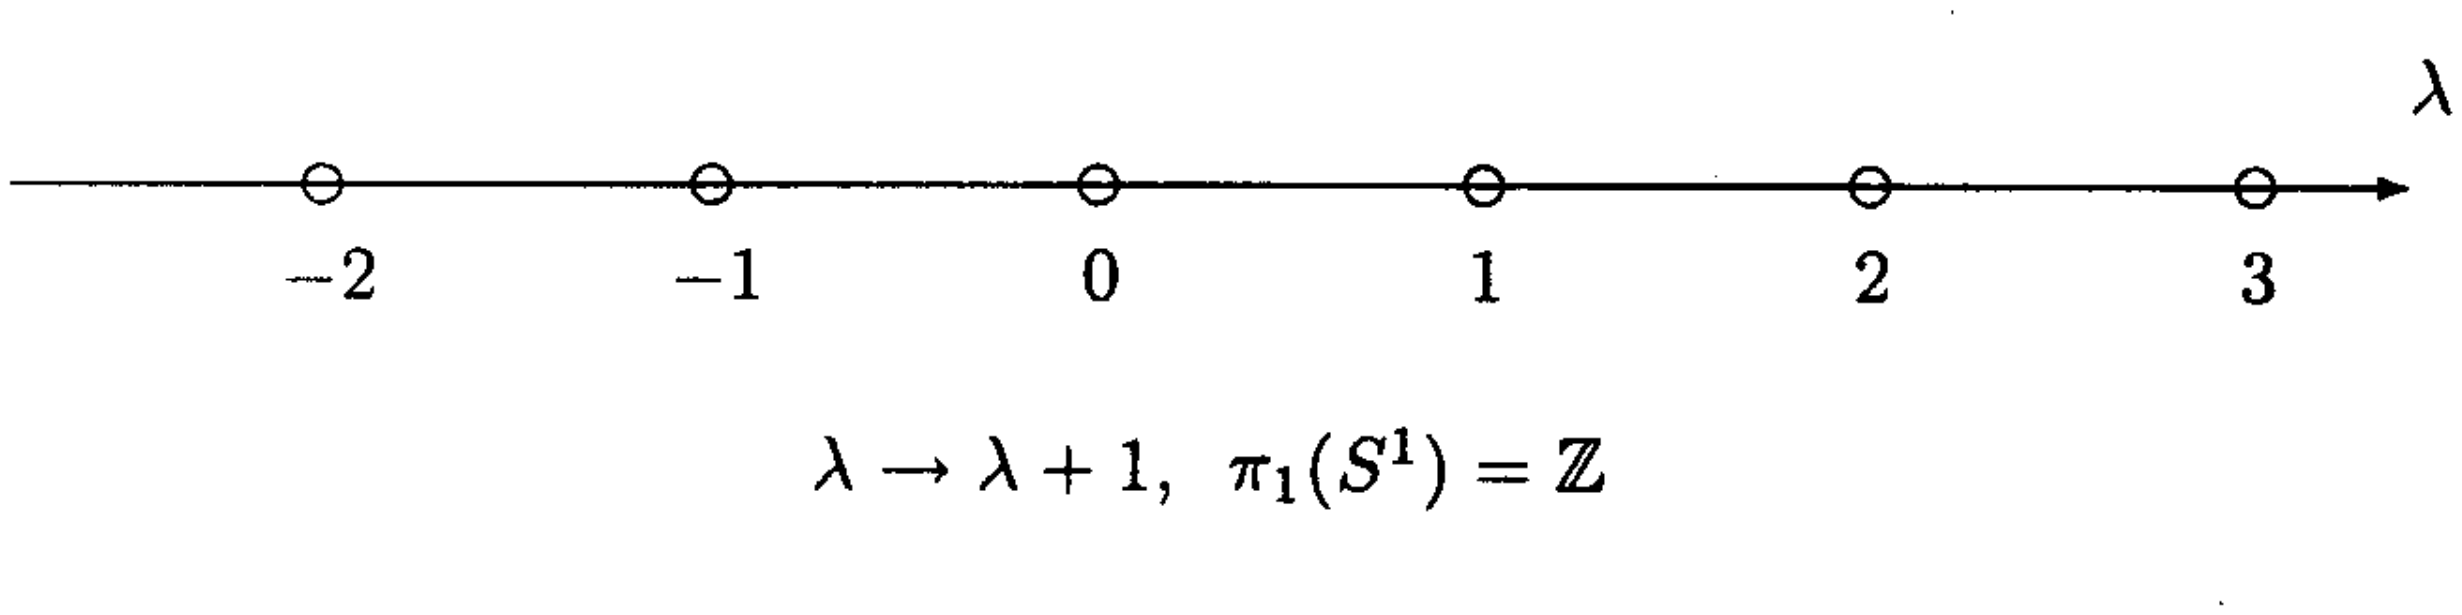
\includegraphics[width=0.72\textwidth]{figures/fig2_19.png}
  \figtitle{2.19}{}
\end{figure}
% [Tutor Note: 例 4 的结论「除 $\pi_1$ 外全为零」是环面的关键性质，证明路线正是 (4.8)：$T^n$ 的万有覆叠 $\R^n$ 可缩，故 $i>1$ 时 $p_*:\pi_i(\R^n)\to\pi_i(T^n)$ 两端为零而给出 $\pi_i(T^n)=0$。图 2.19 画的是 $n=1$ 的模型：直线 $\R$ 上的平移 $\lambda\to\lambda+1$ 给出 $S^1=\R/\Z$。]

% [原文 p.37]
\begin{example}{5}
在同胚意义下，每个闭的可定向曲面都是带把手的球面（见图 2.20）。这个事实由 Möbius 确立。我们把粘上 $g$ 个把手的球面记作 $M_g^2$；整数 $g$ 称为\emph{亏格}。对 $g\ge2$，每个曲面 $M_g^2$ 都可以作为 Lobachevsky 平面 $L^2$ 在某群 $\Gamma$ 的（保度量）变换之离散自由作用下的轨道空间而得到（见图 2.21，其中 $L^2$ 表示为单位圆盘的内点）。
\begin{figure}[htbp]
  \centering
  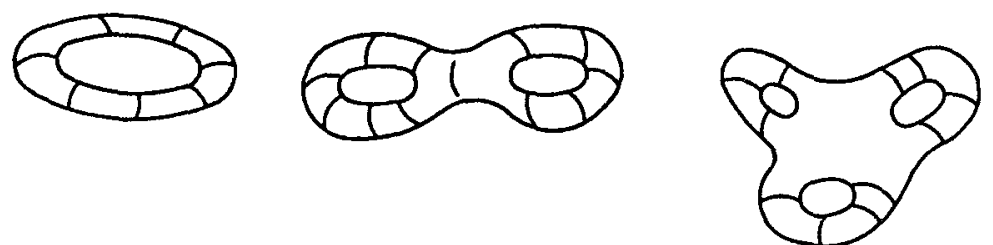
\includegraphics[width=0.46\textwidth]{figures/fig2_20.png}
  \figtitle{2.20}{(a) $g=1$；(b) $g=2$；(c) $g=3$}
\end{figure}
对 $L^2$ 的上半平面模型 $\operatorname{Im}z>0$，群 $\Gamma$ 可以取为由下列 $2g$ 个分式线性变换 $A_1,\dots,A_{2g}:L^2\to L^2$（它们都保持该半平面）生成的群：
\begin{figure}[htbp]
  \centering
  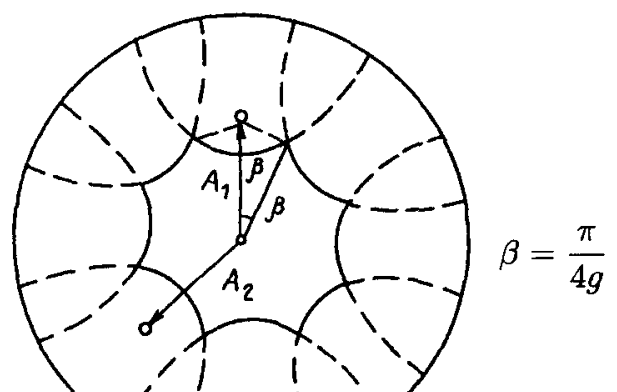
\includegraphics[width=0.50\textwidth]{figures/fig2_21.png}
  \figtitle{2.21}{}
\end{figure}
\noindent{\small 图中注记：变换 $A_1$ 与 $A_2$ 把八边形的中心移到箭头所指的点。}

\begin{equation}
  \begin{gathered}
    A_1=\begin{pmatrix} e^l & 0\\ 0 & e^{-l}\end{pmatrix},\qquad
    A_k=B_g^{-k+1}A_1B_g^{k-1},\\[2pt]
    B_g=\begin{pmatrix} \cos\alpha & \sin\alpha\\ -\sin\alpha & \cos\alpha\end{pmatrix},\qquad
    l=\ln\frac{\cos\beta+\sqrt{\cos2\beta}}{\sin\beta},\\[2pt]
    \alpha=\pi\frac{2g-1}{4g},\qquad \beta=\frac{\pi}{4g}.
  \end{gathered}
  \tag{4.17}
\end{equation}
% [原文 p.38]
（这里矩阵 $\begin{pmatrix} a & b\\ c & d\end{pmatrix}$ 表示分式线性变换
\[
  z\mapsto\frac{az+b}{cz+d}.
\]
图 2.21 画出了其中一部分变换转换到 $L^2$ 的单位圆盘模型后的情形。）可以验证
\begin{equation}
  A_1\cdots A_{2g}A_1^{-1}\cdots A_{2g}^{-1}=1, \tag{4.18}
\end{equation}
并且可以证明 $A_1,\dots,A_{2g}$ 之间的所有关系都是 (4.18) 的推论。于是 $\pi_1(M_g^2)$ 同构于以 $A_1,\dots,A_{2g}$ 为生成元、以单个定义关系 (4.18) 定义的群。也可以为群 $\pi_1(M_g^2)$ 找到另一组生成元 $a_1,\dots,a_g,b_1,\dots,b_g$，使该群只有单个定义关系：
\begin{equation}
  a_1b_1a_1^{-1}b_1^{-1}a_2b_2a_2^{-1}b_2^{-1}\cdots
  a_gb_ga_g^{-1}b_g^{-1}=1. \tag{4.19}
\end{equation}
在这个变换群作用下取轨道空间，其效果本质上就是等同 $L^2$ 中一个 $4g$ 边形（$g=1$ 时在 $\R^2$ 中）的相应边——见图 2.22。\end{example}

\begin{figure}[htbp]
  \centering
  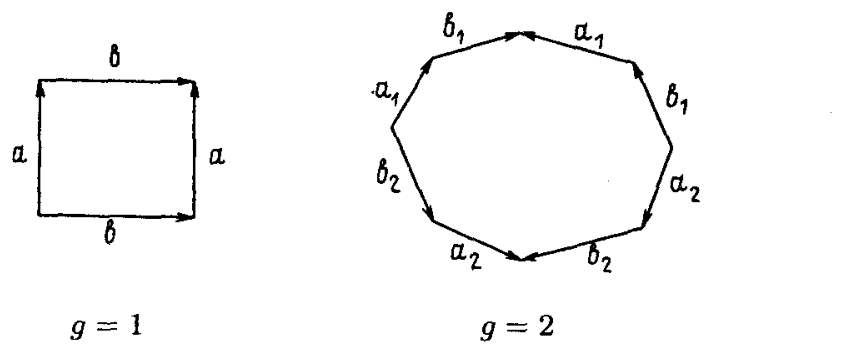
\includegraphics[width=0.66\textwidth]{figures/fig2_22.png}
  \figtitle{2.22}{$g=1$（左，四边形）与 $g=2$（右，八边形）的边等同}
\end{figure}
% [Tutor Note: (4.18) 与 (4.19) 是同一个群 $\pi_1(M_g^2)$ 的两个「呈现」：(4.18) 用 $2g$ 个生成元配一个乘积式关系，(4.19) 用 $2g$ 个生成元配标准的换位子积，后者更常用，因为它直接对应 $4g$ 边形的边配对。$A_k$ 的定义 $A_k=B_g^{-k+1}A_1B_g^{k-1}$ 说明这些变换都是 $A_1$ 在 $B_g$ 的旋转下的共轭，故几何上只有「一个」变换被反复使用。]

\begin{example}{6}
闭的不可定向曲面可以由可定向曲面出发，取后者在 $\Z/2$ 的适当离散自由作用下的轨道空间得到，这与前面描述的从 $S^2$ 构造 $\RP^2$ 类似。由此得到两族不可定向闭曲面：$N_{g,1}^2$ 与 $N_{g,2}^2$。
它们也可以分别由 $4g$ 边与 $4g+2$ 边的多边形经过适当地等同边而得到——见图 2.23。可以为 $\pi_1(N_{g,1}^2)$ 找到生成元 $a_1,\dots,a_g,b_1,\dots,b_g$，使该群只有单个定义关系：
\begin{equation}
  N_{g,1}^2:\quad a_1b_1a_1^{-1}b_1^{-1}\cdots
  a_{g-1}b_{g-1}a_{g-1}^{-1}b_{g-1}^{-1}a_gb_ga_g^{-1}b_g=1. \tag{4.20}
\end{equation}
另一方面，对 $N_{g,2}^2$，群 $\pi_1(N_{g,2}^2)$ 由生成元 $a_1,\dots,a_g,b_1,\dots,b_g,c$ 以及单个定义关系
% [原文 p.39]
\begin{equation}
  N_{g,2}^2:\quad\Bigl(\prod_{i=1}^g a_ib_ia_i^{-1}b_i^{-1}\Bigr)c^2=1 \tag{4.21}
\end{equation}
给出。这两族穷尽了闭的不可定向曲面，这一事实最早由 Poincaré 确立。
\end{example}

\begin{figure}[htbp]
  \centering
  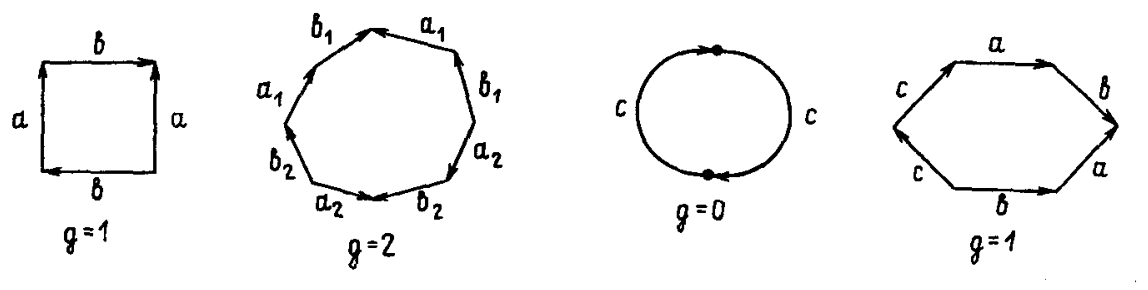
\includegraphics[width=0.86\textwidth]{figures/fig2_23.png}
  \figtitle{2.23}{(a) $N_{g,1}^2$，$g\ge1$（左：Klein 瓶）；(b) $N_{g,2}^2$，$g\ge0$（右：射影平面）}
\end{figure}
% [Tutor Note: (4.20) 末项是 $a_gb_ga_g^{-1}b_g$，最后一个 $b_g$ 不带逆，这不是笔误：不可定向曲面 $N_{g,1}^2$ 的标准关系正是「$g-1$ 个换位子外加 $a_gb_ga_g^{-1}b_g$」；若把末项也写成换位子，所得群就变成可定向曲面 $M_g^2$ 的基本群了。]

可以证明，对一切 2 维流形（即曲面），无论开或闭，只要它不是 $\RP^2$ 也不是 $S^2$，其所有高阶同伦群都平凡：
\begin{equation}
  \pi_i(M^2)=0\quad\text{对 } i>1,\qquad M^2\ne\RP^2,\ S^2. \tag{4.22}
\end{equation}
若一个空间 $X$ 除一个同伦群外其余同伦群都平凡，则称它为 \emph{Eilenberg--MacLane 空间}；当
\begin{equation}
  \pi_n(X)\cong\pi,\qquad \pi_i(X)=0\quad\text{对 } i\ne n \tag{4.23}
\end{equation}
时记作 $K(\pi,n)$。（事实上 $K(\pi,n)$ 可以实现为「CW 复形」——见下文。）我们已经遇到过 $K(\pi,1)$ 型的空间。特别要注意，例 2 末尾提到的空间 $\RP^\infty$ 是 $K(\Z/2,1)$ 型的。\hfill$\square$
% [Tutor Note: (4.22) 是曲面拓扑「只用基本群就够了」的根据：除 $S^2$ 与 $\RP^2$ 外，曲面的万有覆叠可缩，于是 $\pi_i=0$（$i>1$）。也正因如此，闭曲面的分类可以完全由 $\pi_1$ 的群论呈现来完成（例 5、例 6 的 (4.19)–(4.21)），而 $S^2$、$\RP^2$ 因有 $\pi_2=\Z$ 必须单独处理。]

\begin{example}{7}
\emph{Hopf 纤维化}。$n$ 个复维的复射影空间 $\CP^n$ 仿照 $\RP^n$ 定义：把 $\C^{n+1}$ 中的非零向量，若彼此相差一个非零复纯量倍，则等同起来：
\[
  (\lambda^0,\dots,\lambda^n)\sim(\lambda\lambda^0,\dots,\lambda\lambda^n),
  \qquad \lambda\in\C,\ \lambda\ne0.
\]
只限于 $\C^{n+1}$ 中满足
\[
  \sum_j|\lambda^j|^2=1
\]
的那些点，我们推出 $\CP^n$ 可以实现为圆周群 $S^1\cong U(1)\cong\SO_2$ 在 $S^{2n+1}$ 上的自由作用的轨道空间，该作用由
\[
  (\lambda^0,\dots,\lambda^n)\to(e^{i\alpha}\lambda^0,\dots,e^{i\alpha}\lambda^n)
\]
给出。这就定义了 \emph{Hopf 纤维化}：$p:S^{2n+1}\to\CP^n$，其纤维为 $S^1\cong U(1)\cong\SO_2$。由于 $\pi_1(S^1)\cong\Z$、$i>1$ 时 $\pi_i(S^1)=0$（见上文），由纤维化的正合列（见 (4.7)）得到下列同构：
% [原文 p.40]
\begin{equation}
  \begin{gathered}
    \pi_i(S^{2n+1})\cong\pi_i(\CP^n),\qquad i\ne2,\\
    \pi_{2n+1}(S^{2n+1})\cong\pi_{2n+1}(\CP^n)\cong\Z,\\
    \pi_2(\CP^2)\cong\Z\cong\pi_1(S^1).
  \end{gathered}
  \tag{4.24}
\end{equation}
令 $n\to\infty$ 取直接极限可知，无限维复射影空间 $\CP^\infty$ 具有 Eilenberg--MacLane 空间 $K(\Z,2)$ 的型。由 (4.24) 以及 $\CP^1\cong S^2$ 这一事实，我们还推出 \emph{Hopf 定理}：
\begin{equation}
  \pi_3(S^2)\cong\Z. \tag{4.25}
\end{equation}
\end{example}
% [Tutor Note: (4.24) 的中间一行要单独看：$p_*:\pi_{2n+1}(S^{2n+1})\to\pi_{2n+1}(\CP^n)$ 是同构，而 $\pi_{2n+1}(\CP^n)\cong\Z$ 由 (4.7) 里 $\pi_{2n+1}(S^1)=0$ 与 $\pi_{2n}(S^1)=0$ 夹出。注意 $\CP^n$ 是 $2n$ 维实流形，$\pi_{2n+1}$ 已超出维数，这里全靠纤维化的长正合列。(4.25) 的 $\pi_3(S^2)\cong\Z$ 是 Hopf 用 $S^3\to S^2$ 的 Hopf 映射算出的第一个非平凡高阶同伦群。]

\begin{example}{8}
考虑一个纽结，即嵌入 3 维球面 $S^3$ 中的圆周 $S^1$，以及它的补集 $S^3\setminus S^1=U$。（前面我们考虑的是 $\R^3$ 中的纽结；这里加上了一个无穷远点，以得到紧空间 $S^3$。）Papakyriakopoulos 的一个定理断言 $\pi_2(U)=0$，由此不难证明 $j>2$ 时 $\pi_j(U)=0$。因此纽结补集全都是 $K(\pi,1)$ 型的 Eilenberg--MacLane 空间。
\end{example}

最后我们指出，在 $K(\pi,n)$ 型空间的简单而著名的例子中，只有一个是 $n>1$ 的，即 $K(\Z,2)=\CP^\infty$。就代数拓扑的工具而言，绝大多数场合只需 $K(\pi,n)$ 的\emph{存在性}就够了；只有在一篇重要论文（E. Cartan 的）中，才实质性地用到了某个具体的代数模型。
% CHUNK ch02c DONE
